\begin{frame}{Dychotomia CSP}

\begin{columns}
\column{0.65\textwidth}
    \!\textcolor{cfblue}{Dychotomia CSP (Bulatov, Zhuk; 2017)} \\
    Dla grafu \(H\) problem CSP\((H)\) albo jest w P, albo~NP-zupełny. \\
    \vspace{1.5em}
    \onslide<3->{
        U nas \(H\) jest spójny i gładki.
    }

\column{0.35\textwidth}
    \begin{figure}[H]
        \centering
        \begin{tikzpicture}[
    scale=1.25,
    line width=1pt
]

% Jeśli P \cap NP-hard = \emptyset to P\neq NP
% ----------- NP ------------
\draw (0,0) ellipse (1.75 and 1.45);
\node at (1.2,0) {\large NP};

% ------- NP-complete -------
\draw (0,0.75) ellipse (0.8 and 0.55);
\node at (1.4,1.75) {\large NP-zupełne};
\draw (1.35,1.45) -- (0.5,0.8);

% ------------ P ------------
\draw (0,-0.75) ellipse (0.8 and 0.55);
\node at (0.4,-0.8) {\large P};

% ----------- CSP -----------
\begin{scope}[line width=1.6pt, rounded corners=8pt, cfblue]
\only<1>{
    \draw (-0.55,-1) rectangle (0,1);
    \node at (-1.1,0) {\Large CSP};
}

\only<2->{
    \draw (-0.55,0.4) rectangle (0,1);
    \draw (-0.55,-1) rectangle (0,-0.4);
    \node at (-1.1,0) {\Large CSP};
}
\end{scope}

\end{tikzpicture} 
    \end{figure}
    \vspace{1em}

\end{columns}

\end{frame}

% --------------------------------------------------------------

\begin{frame}{Rozważamy dużą klasę grafów}

\begin{figure}
    \centering
    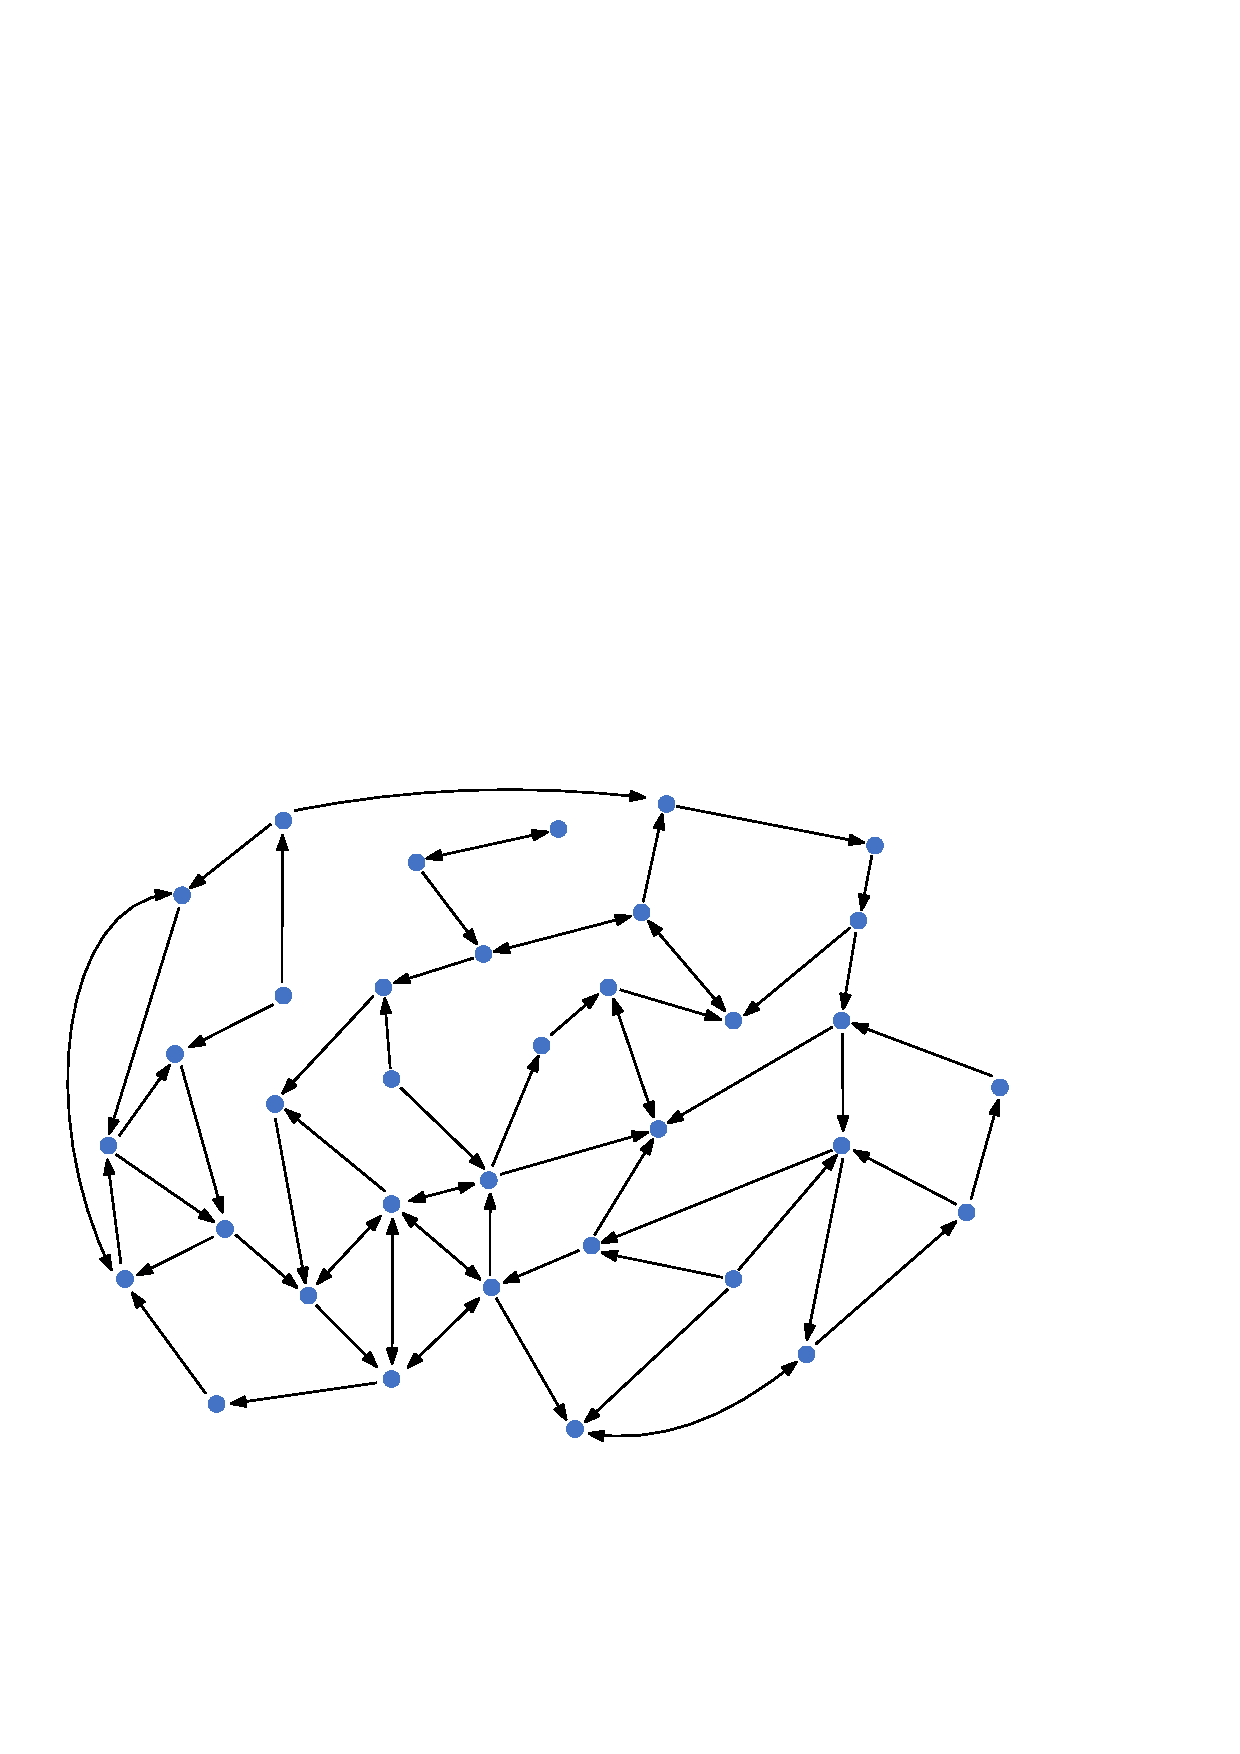
\includegraphics[width=0.6\linewidth]{img/random.pdf}
\end{figure}
    
\end{frame}